\chapter{Le Machine Learning}

Dans le cadre du rapport de stage, je vais me focaliser sur l'approche \textit{représentation et raisonnement}.\\
\linebreak
Un \textit{Dataset} est un tableau représentant pour chaque colonne une donnée et pour chaque ligne un \textit{sample}, les samples sont composés d'une et d'une seule valeur par colonne, cette valeur peut être n'importe quoi (chaine de caractère, tableau, entier, boolean, ...). Un des formats les plus utilisés pour illustrer la table est le format \textit{csv}, \textit{SQL} ou \textit{excel}.\\
\pagebreak

\section{Les premiers pas}

Dans les années 1950, on ne parlait pas encore du \textit{Machine Learning} que l'on n'a maintenant, on parlait de méthode de généralisation d'un modèle.\\
Imaginons que vous vouliez prédire un résultat de type boolean à partir de données que vous avez enregistré.

\begin{center}
\begin{multicols}{3}
[Sans tout ses algorithmes de machines learning actuel, le principe était de généraliser le modèle au maximum,pour ceci avec un trahit puis pour chaque ligne faire l'intersection avec le trahit, tout ceci donne $\crouge{c}$:]

\begin{tabular}{ccc|c}
A & B & C & résultat \\
\hline
0 & 0 & 1 & 1\\
0 & 1 & 1 & 1\\
1 & 1 & 0 & 0\\
\end{tabular}
\scalebox{0.4}{
\begin{tikzpicture}[->,>=stealth',shorten >=1pt,auto,node distance=2.8cm,
                    semithick]
  \tikzstyle{every state}=[fill=white,draw=none,text=black]

  \node[state]         (Z)                    {$\{\}$};
  \node[state]         (B) [below  of=Z]      {$B$};
  \node[state]         (A) [left  of=B]       {$A$};
  \node[state]         (C) [right of=B]       {$\crouge{C}$};
  \node[state]		   (AB) [below of=A]      {$AB$};
  \node[state]		   (AC) [right of=AB]     {$AC$};
  \node[state]         (BC) [right of=AC]     {$BC$};
  \node[state] 		   (ABC) [below of=AC]    {$ABC$};
  

  \path (Z) edge              node {} (A)
            edge              node {} (B)
            edge			  node {} (C)
        (A) edge			  node {} (AB)
        	edge			  node {} (AC)
        (B) edge			  node {} (AB)
        	edge			  node {} (BC)
        (C) edge 			  node {} (AC)
        	edge			  node {} (BC)
        (AB) edge 			  node {} (ABC)
        (AC) edge			  node {} (ABC)
        (BC) edge			  node {} (ABC);
\end{tikzpicture} }
\end{multicols}
\end{center}

Cette technique, beaucoup utilisé en fouille de données, a ses limites, quelques années plus tard vient les premiers algorithmes de machine learning qui de nos jours sont encore bien répandu, en voici une liste non exhaustif:

\begin{description}
\item[Gradient]: Pour un nuage de points, le but est de trouver une droite qui minimise la distance (sur l'axe Y) entre celle ci et chaque  points du nuage.
\item[Kmeans]: Pour chaque sample du dataset, le but est de former des groupes de samples qui se ressemble le plus.
\end{description}

Ci dessus, deux modèles du machine learning, le Gradient est un modèle dit \textit{Supervisé} et le Kmeans est dit \textit{Non Supervisé}. La différence entre les deux modèles et simple, soit un dataset possédant une colonne nommée \textit{Étiquette} (ou Class en anglais) donne le résultat du sample concerné, il est donc facile pour un sample possédant une colonne Étiquette de connaitre son appartenance, on dit alors que le modèle est supervisé, pour un modèle non supervisé, nous ne connaissons pas les étiquettes des samples.\\
\pagebreak

\section{Algorithmes d'apprentissage}

De nos jours il existe une tonne d'algorithme d'apprentissage, tout ont plus ou moins leurs utilités, avantage, faiblesse, d'où le fait que pour le data scientiste doit essayer un peu tous les algorithmes et de juger de leur efficacité via les résultats données. Bien-sûr si un Gradient suffit pourquoi vouloir utiliser un réseau de neurones.\\
En voici une liste non exhaustive utilisé lors du stage à des fins de teste (via la librairie sci-kit-learn de python):

\begin{description}
\item[Support Vector Machine]: Le support vector machines cherche un hyperplan (de couleur noir) pouvant départager des classes,
Il en existe une infinité d'hyperplan qui peuvent les départager, donc introduisons un autre concept, celui de 
l'hyperplan qui maximise la séparation entre les deux classes (les droites $\corange{Oranges}$ appelé $Margin$.\\
\cshape{0.5}{
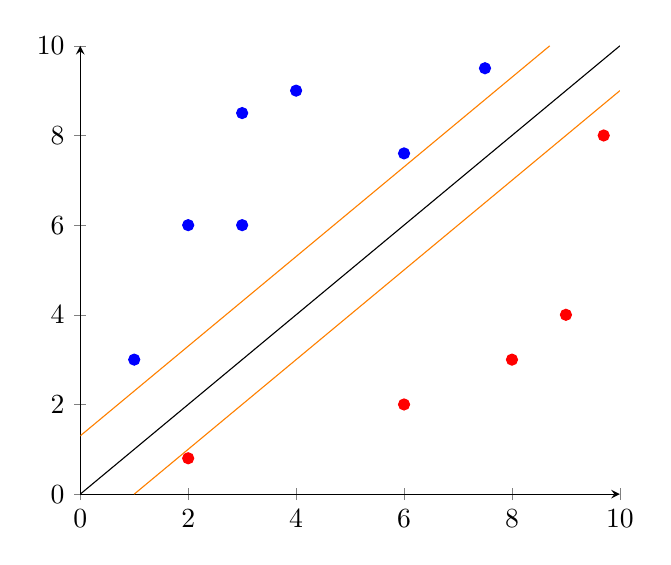
\begin{tikzpicture}
  \begin{axis} [
      axis lines = left,
      xmin       = 0,
      ymin       = 0,
    ]
    \addplot [color=black] coordinates {(0,0)(10,10)};
    \addplot [color=orange] coordinates {(0,1.3)(8.7,10) };
    \addplot [color=orange] coordinates {(1,0)(10,9) };
    \addplot [only marks, mark=*, color=blue] coordinates {(2,6)(1,3)(6,7.6)(3,8.5)(7.5,9.5)(4,9)(3,6)};
    \addplot [only marks, mark=*, color=red]  coordinates {(2,0.8)(6,2)(9,4)(9.7,8)(8,3)};
  \end{axis}
\end{tikzpicture}
}

\item[Decision Tree]: Un arbre de décision est une suite de nœuds relié par au moins une arrête, on emprunte une arrête par rapport à la décision qui est à prendre via le nœuds courant. L'ordre des nœuds est choisis selon des critères (les trois les plus utilisé sont \textit{Entropy}, \textit{Information grain} et \textit{Gini}), ces trois critères de sélection appliqué au même dataset peut donner un arbre diffèrent. Une feuille d'arbre est un nœuds n'ayant aucun fils, les étiquettes des prédictions s'y trouve.
\cshape{0.5}{
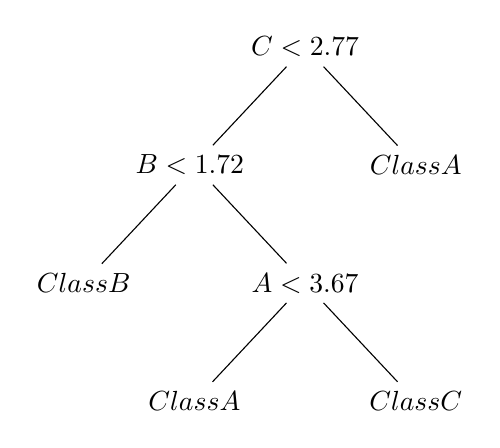
\begin{tikzpicture}[sibling distance=8em,
  every node/.style = {scale=1,
    draw=none, align=center}]]
  \node {$C < 2.77$}
 	  child { node {$B < 1.72$ }
 	    child { node {$Class B$}}
 	    child { node {$A < 3.67$}
 	      child { node {$Class A$}
 	      }
 	      child { node {$Class C$} }
 	    }
 	  }
 	  child { node {$Class A$} }
    ;
\end{tikzpicture}
}
\end{description}

\pagebreak
Traiter les samples de type numérique donne beaucoup de possibilités de traiter un problème.\\
L'évolution a fait que de plus de données sont de type textuel, pour des dates et durées, le problème reste simple à résoudre, pour une suite de mots fini, il suffit de les énumérer, mais pour les données du langage naturel?\\
\linebreak

\section{Langage naturel}

Un texte peut être long ou court, contenant des liens, des caractères spéciaux, on ne peut pas utiliser lancer un algorithme comme ci dessus sur des textes et en espérer en tirer de bons résultats, plusieurs étapes sont nécessaires pour pouvoir utiliser des algorithmes qui travaillent avec des textes. 

\subsection{Génération de texte}
La génération de texte peut être aléatoire ou provenant d'aucune source, mais ce n'est pas le sujet, restons proche des missions abordées en stage. Les deux méthodes de génération de texte ci dessous font appel à beaucoup d'algorithmes de machine learning pour créer un modèle d'interprétation des entrées.

\begin{description}
\item[Optical Caracteres Reconization]: Le but est de lire les caractères présents sur du support physique, des feuilles de papier, des photos. Après un traitement de l'image, l'algorithme lisant les entrées utilisent des méthodes de \textit{Deep Learning} pour reconnaitre qu'un motif et un caractère. Puis l'algorithme va faire des prédictions vua ce qu'il a apprit, il apprend via des samples représentant des représentations vectorielle des caractères. En pratique \textit{Open CV} et \textit{Sklearn ou tensorflow} sont utilisés.

\item[Speech To Text (STT)]: Dans le cadre du stage, nous avons utilisé un de ses algorithmes pour nourrir nos IA, le STT a besoin de beaucoup de données d'entrainement pour pouvoir modéliser le graph du langage souhaité, un sample d'entrainement et tout simplement une piste audio et son transcrit en format textuel, après de longues heures et le graphe généré, nous pouvons entrer de nouvelles pistes audios sans transcrit pour recevoir des prédictions.
\end{description}

\pagebreak
\subsection{Nettoyage des données}

Le français est un langage riche en dérivé de lettres notamment pour ses caractères accentués, le premier travail est de réduire l'espace des caractères en éliminent par exemple les majuscules et les remplacer par des minuscules, éliminer la ponctuation, puis normaliser les accents. Nous pouvons obtenir un texte comme suite:
\\
\sepline\\
Bonjour, je viens parce-que j'ai une fuite d'eau sur mon plafond, j'ai déjà prit contact avec une entreprise pour ses réparations mais elle n'a pas donné suite.\\
\sepline\\
bonjour je viens parce que j ai une fuite d eau sur mon plafond, j ai deja prit contact avec une entreprise pour ses reparations mais elle n a pas donne suite\\
\sepline\\

Selon la documentation de scikit-learn (librairie python) la méthode la plus optimisée serait le \textit{Bag of words},pour chaque document \textit{i}, pour chaque mot du texte \textit{w}, associer un indice unique \textit{j} au mot \textit{w}, et affecter le nombre d'occurrences de \textit{w} dans $List[i,j]$. Transformer toutes les occurrences en fréquences. Une fois ces étapes terminer, nous pouvons utiliser un classifier pour faire des prédictions sur les textes.\\
Lors du stage, selon les testes effectué sur presque 4000 corps de mail de longueur descente et nettoyée pour ne laisser que le contenue pertinent (on n'a aussi enlevé les \textit{stopwords} comme les \textit{le,la,d',...}), 2 algorithmes ont eu des résultats correct, les réseaux  de bayes naïf (et ses dérivé) et le réseau de neurones.\\
\linebreak
Concernant des techniques de nettoyage de données, 2 ETL (Extrac Ttransform Load) ont été essayé, Talend et DataIku, j'ai une préférence pour DataIku étant meilleur en python qu'en java, le même travail peut être fait avec ses deux ETL, mais la librairie de DataIku est bien plus remplit et permet de faire la plupart des traitements sur le Data sans écrire une ligne de code, là où Talend le code est quasiment omniprésent. De plus la où Talend s'arrête sur le traitement et la transformation des données, DataIku permet d'exécuter des algorithmes de Machine Learning, tous ses algorithmes sont issu du paquet scikit-learn.
\pagebreak

\sepline\\
Plus haut j'ai parlé de Machine learning, de traitement des chaines textuels, de génération de chaines textuels, ce qui une fois additionné fait une jolie intelligence artificielle qui pour un besoin peut nous répondre ce qu'il faut. Prenons un exemple présent dans certains films qui se veulent futuriste, tient prenons le film \textit{Her} sortie en 2013.\\
\linebreak
Pour faire très court et rester dans le sujet du stage, le personnage principal du film nommé Theodore devenais ami avec un système d'exploitation (os) nommé Amy, une os tellement proche de l'être humain, celle ci pouvais apprendre, comprendre et communiquer sans aucun problème avec Theodore.\\
Comme quoi qu'avec un Speech To Text et de bons algorithmes nous pouvons créer un processus qui simule la conscience d'un humain. Prendre par exemple un film n'est pas très pertinent, car tout est réalisable avec de l'argent, revenons dans la vrai vie. Un outil présent dans le monde de L'IOT (internet des objets) qui justement commence à bien se développer, Commencé en 2008 par Google et largement plus connu sous la firme Apple, je parle bien des logiciel ou objets de reconnaissance vocal.\\
\linebreak
La reconnaissance vocal passe son temps à écouter son environnement et à traduire ce qu'elle peut prendre comme étant de la parole en chaine de caractère, les intérêts ne sont pas multiple, la plus part du temps c'est pour simplifier la vie des utilisateurs, "Quelle sera la Méteo pour demain.", "Comment préparer des cookies", "Appeler Papa". L'utilisateur fait des requêtes à son logiciel qui lui va transformer l'information en chaine de caractère qui lui va faire une requête ailleurs. On peut comparer la reconnaissance vocal comme des requêtes en base de données, la base de données étant internet. 